% \documentclass[fleqn,xcolor=dvipsnames]{beamer}
\PassOptionsToPackage{unicode}{hyperref}
\PassOptionsToPackage{naturalnames}{hyperref}
\documentclass[xcolor=table]{beamer}
\usepackage[labelfont={color=red}]{caption}
\usetheme{Boadilla}
\usepackage{ifthen}
% \usetheme{default}
% \usetheme{Warsaw}
% \usetheme{CambridgeUS}
\beamertemplatenavigationsymbolsempty 
\makeatletter
\newcommand{\srcsize}{\@setfontsize{\srcsize}{5pt}{5pt}}
\makeatother
\usepackage{pgffor}

% \usepackage{pgf}

%\usetheme{CambridgeUS}
% \usetheme{Sybila}
% \usetheme[hideothersubsections]{Berkeley}
% \usetheme[hideothersubsections]{PaloAlto}
% \usetheme[hideothersubsections]{Goettingen}
%\usetheme{CambridgeUS}
% \usetheme{Bergen} % This template has nagivation on the left
% \usetheme{Frankfurt} % Similar to the default with an extra region at the top.
\setbeamertemplate{caption}[numbered]
\setbeamerfont{caption}{size=\tiny}
\framesubtitle{<subtitle>}

\hypersetup{
        colorlinks=true,
        linkcolor=,
        filecolor=lightthulianpink,urlcolor=lightthulianpink,
        }
        
\setbeamertemplate{caption}[numbered]
\setbeamerfont{caption}{size=\tiny}
\framesubtitle{<subtitle>}

% Uncomment the following line if you want page numbers and using Warsaw theme%
\setbeamertemplate{footline}[page number]

\definecolor{aggiemaroon}{RGB}{80,0,0} % Official RGB code for aggie maroon
\definecolor{babypink}{rgb}{0.96, 0.76, 0.76}
\definecolor{persianpink}{rgb}{0.97, 0.5, 0.75}
\definecolor{babyblue}{rgb}{0.54, 0.81, 0.94}
\definecolor{SkyBlue}{rgb}{0.309,0.807, 1}
\definecolor{lightcyan}{rgb}{0.88, 1.0, 1.0}
 \usecolortheme[named=babyblue]{structure}
  \setbeamercolor{itemize item}{fg=blue!80!black!}
  \useinnertheme{rounded}
  %\useoutertheme{sidebar}
  \usefonttheme{structurebold}
  %\usefonttheme[onlymath]{serif}
  \setbeamercovered{transparent}
  \setbeamertemplate{blocks}[rounded][shadow=true]
 
	\makeatletter
\setbeamertemplate{footline}
{
    \leavevmode%
    \hbox{%
        \begin{beamercolorbox}[wd=.333333\paperwidth,ht=2.25ex,dp=1ex,center]{author in head/foot}%
            \usebeamerfont{author in head/foot}\insertshortauthor
        \end{beamercolorbox}%
        \begin{beamercolorbox}[wd=.333333\paperwidth,ht=2.25ex,dp=1ex,center]{title in head/foot}%
            \usebeamerfont{title in head/foot}\insertshorttitle
        \end{beamercolorbox}%
        \begin{beamercolorbox}[wd=.333333\paperwidth,ht=2.25ex,dp=1ex,right]{date in head/foot}%
            \usebeamerfont{ in head/foot}\insertshortdate{}\hspace*{2em}
            \insertframenumber{} / \inserttotalframenumber\hspace*{2ex} 
        \end{beamercolorbox}}%
        \vskip0pt%
    }
    \makeatother

\graphicspath{ {../} {../BFSoutput} {../BFSNodes} {../DFSoutput} {../DFSNodes} {../UCSoutput} {../UCSNodes}  }
\usepackage{ragged2e}
\usepackage{amsmath}
\usepackage{caption}
\usepackage{graphicx,comment}
\usepackage[english]{babel}
\usepackage{graphicx}
\usepackage{rotating}
\usepackage{multicol}
\usepackage{hyperref}
\usepackage{enumerate}
\usepackage{tikz}
\usepackage{graphicx}
\usepackage{bm}
\usepackage{wrapfig}
\usepackage{float}
\usepackage{multirow}
\usepackage{adjustbox}
\usepackage{xparse, minted}



\definecolor{colorHighlight}{rgb}{0.917,0.96,0.101}

\newcommand{\drawMineUnvisited}[1]{\draw [lightgray, fill=lightgray, fill opacity=0.5] #1 circle [radius=0.4]}
\newcommand{\drawMineFrontier}[1]{\draw [SkyBlue, fill=SkyBlue, fill opacity=0.5] #1 circle [radius=0.4]}
\newcommand{\drawMineVisited}[1]{\draw [orange, fill=orange, fill opacity=0.5] #1 circle [radius=0.4]}
\newcommand{\drawMineFound}[1]{\draw [green, fill=green, fill opacity=0.5] #1 circle [radius=0.4]}
\newcommand{\drawMineNotFound}[1]{\draw [black, fill=black, fill opacity=0.9] #1 circle [radius=0.4]}


\newenvironment{MyMinted}
{\VerbatimEnvironment\begin{minted}[bgcolor=lightgray]{octave}}{\end{minted}} 

\title[Artificial Intelligence]{Artificial Intelligence} % The short title appears at the bottom of every slide, the full title is only on the title page

\author[Narendiran]{Narendiran S} % Your name\\

\institute[NIT Calicut] % Your institution as it will appear on the bottom of every slide, may be shorthand to save space
{Department of Electronics and Communication Engineering\\
National Institute of Technology, Calicut\\
}



\AtBeginSection[]
{
  \begin{frame}<beamer>
    \frametitle{Section \thesection}
    \tableofcontents[currentsection,currentsubsection]
  \end{frame}
}

\begin{document}

\begin{frame}
\titlepage
\end{frame}

\begin{frame}{Assumptions}
  \begin{itemize}
    \item Gray color represents Unvisited Node.
    \item Blue color represents Notes in Frontier.
    \item Orange color represents Visited Nodes.
    \item Black color represents Failure Nodes.
    \item Green color represents Success Node.
  \end{itemize}
  \vspace*{0.5cm}
  \begin{center}
    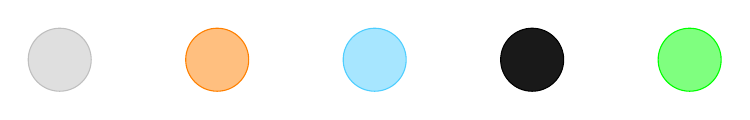
\begin{tikzpicture}
      \drawMineUnvisited{(-4,0)};
      \drawMineVisited{(-2,0)};
      \drawMineFrontier{(0,0)};     
      \drawMineNotFound{(2,0)};
      \drawMineFound{(4,0)};
    \end{tikzpicture}
  \end{center}
\end{frame}

\begin{frame}
The map I choose is Tamil Nadu.
The path is from \emph{Coimbatore} to \emph{Pondicherry}.
\begin{figure}[H]
\includegraphics[height=0.9\textheight]{tamilNaduOutlinePath.jpg}
\end{figure}
\end{frame}


\section*{BFS}
\begin{frame}[fragile]{Breath First Search - BFS}
  \begin{itemize}
    \item In BFS, we expand the shallowest node first.
    \item It doesn't use any domain information.
    \item The data structure used is a \textbf{QUEUE}.
  \end{itemize}
  \footnotesize
  \begin{MyMinted}
    function BREADTH-FIRST-SEARCH(initialState, goalTest)
      returns SUCCESS or FAILURE:

      frontier = Queue.new(initialState)
      explored = Set.new()

      while not frontier.isEmpty()
        state = frontier.dequeue()
        explored.add(state)
        if goalTest(state):
          return SUCCESS(state)

        for neighbor in state.neighbors():
          if neighbor not in frontier U explored:
            frontier.enqueue(neighbor)
      return FAILURE
  \end{MyMinted}
\end{frame}


\begin{frame}
  { \tiny Fontier: ['Coimbatore'] }
  \includegraphics[width=1\textwidth]{../BFSNodes/2-1.png}
  \begin{center}
    \includegraphics[height=0.6\textheight]{../BFSoutput/tamilBFS0.jpg}
  \end{center}
\end{frame}
\begin{frame}
  { \tiny Fontier: ['Dindigul', 'Erode', 'Karur', 'Nilgiris', 'Tiruppur'] }
  \includegraphics[width=1\textwidth]{../BFSNodes/3-1.png}
  \begin{center}
    \includegraphics[height=0.6\textheight]{../BFSoutput/tamilBFS1.jpg}
  \end{center}
\end{frame}
\begin{frame}
  { \tiny Fontier: ['Erode', 'Karur', 'Nilgiris', 'Tiruppur', 'Madurai', 'Theni', 'Trichy'] }
  \includegraphics[width=1\textwidth]{../BFSNodes/4-1.png}
  \begin{center}
    \includegraphics[height=0.6\textheight]{../BFSoutput/tamilBFS2.jpg}
  \end{center}
\end{frame}
\begin{frame}
  { \tiny Fontier: ['Karur', 'Nilgiris', 'Tiruppur', 'Madurai', 'Theni', 'Trichy', 'Salem'] }
  \includegraphics[width=1\textwidth]{../BFSNodes/5-1.png}
  \begin{center}
    \includegraphics[height=0.6\textheight]{../BFSoutput/tamilBFS3.jpg}
  \end{center}
\end{frame}
\begin{frame}
  { \tiny Fontier: ['Nilgiris', 'Tiruppur', 'Madurai', 'Theni', 'Trichy', 'Salem', 'Namakkal'] }
  \includegraphics[width=1\textwidth]{../BFSNodes/6-1.png}
  \begin{center}
    \includegraphics[height=0.6\textheight]{../BFSoutput/tamilBFS4.jpg}
  \end{center}
\end{frame}
\begin{frame}
  { \tiny Fontier: ['Tiruppur', 'Madurai', 'Theni', 'Trichy', 'Salem', 'Namakkal'] }
  \includegraphics[width=1\textwidth]{../BFSNodes/7-1.png}
  \begin{center}
    \includegraphics[height=0.6\textheight]{../BFSoutput/tamilBFS5.jpg}
  \end{center}
\end{frame}
\begin{frame}
  { \tiny Fontier: ['Tiruppur', 'Madurai', 'Theni', 'Trichy', 'Salem', 'Namakkal'] }
  \includegraphics[width=1\textwidth]{../BFSNodes/8-1.png}
  \begin{center}
    \includegraphics[height=0.6\textheight]{../BFSoutput/tamilBFS6.jpg}
  \end{center}
\end{frame}
\begin{frame}
  { \tiny Fontier: ['Madurai', 'Theni', 'Trichy', 'Salem', 'Namakkal'] }
  \includegraphics[width=1\textwidth]{../BFSNodes/9-1.png}
  \begin{center}
    \includegraphics[height=0.6\textheight]{../BFSoutput/tamilBFS7.jpg}
  \end{center}
\end{frame}
\begin{frame}
  { \tiny Fontier: ['Madurai', 'Theni', 'Trichy', 'Salem', 'Namakkal'] }
  \includegraphics[width=1\textwidth]{../BFSNodes/10-1.png}
  \begin{center}
    \includegraphics[height=0.6\textheight]{../BFSoutput/tamilBFS8.jpg}
  \end{center}
\end{frame}
\begin{frame}
  { \tiny Fontier: ['Theni', 'Trichy', 'Salem', 'Namakkal', 'Ramanathapuram', 'Sivagangai', 'Tenkasi', 'Thoothukudi', 'Virudunagar'] }
  \includegraphics[width=1\textwidth]{../BFSNodes/11-1.png}
  \begin{center}
    \includegraphics[height=0.6\textheight]{../BFSoutput/tamilBFS9.jpg}
  \end{center}
\end{frame}
\begin{frame}
  { \tiny Fontier: ['Trichy', 'Salem', 'Namakkal', 'Ramanathapuram', 'Sivagangai', 'Tenkasi', 'Thoothukudi', 'Virudunagar'] }
  \includegraphics[width=1\textwidth]{../BFSNodes/12-1.png}
  \begin{center}
    \includegraphics[height=0.6\textheight]{../BFSoutput/tamilBFS10.jpg}
  \end{center}
\end{frame}
\begin{frame}
  { \tiny Fontier: ['Trichy', 'Salem', 'Namakkal', 'Ramanathapuram', 'Sivagangai', 'Tenkasi', 'Thoothukudi', 'Virudunagar'] }
  \includegraphics[width=1\textwidth]{../BFSNodes/13-1.png}
  \begin{center}
    \includegraphics[height=0.6\textheight]{../BFSoutput/tamilBFS11.jpg}
  \end{center}
\end{frame}
\begin{frame}
  { \tiny Fontier: ['Salem', 'Namakkal', 'Ramanathapuram', 'Sivagangai', 'Tenkasi', 'Thoothukudi', 'Virudunagar', 'Pudukottai', 'Tanjavur'] }
  \includegraphics[width=1\textwidth]{../BFSNodes/14-1.png}
  \begin{center}
    \includegraphics[height=0.55\textheight]{../BFSoutput/tamilBFS12.jpg}
  \end{center}
\end{frame}
\begin{frame}
  { \tiny Fontier: ['Namakkal', 'Ramanathapuram', 'Sivagangai', 'Tenkasi', 'Thoothukudi', 'Virudunagar', 'Pudukottai', 'Tanjavur', 'Cuddalore', 'Dharmapuri', 'Villupuram'] }
  \includegraphics[width=1\textwidth]{../BFSNodes/15-1.png}
  \begin{center}
    \includegraphics[height=0.55\textheight]{../BFSoutput/tamilBFS13.jpg}
  \end{center}
\end{frame}
\begin{frame}
  { \tiny Fontier: ['Ramanathapuram', 'Sivagangai', 'Tenkasi', 'Thoothukudi', 'Virudunagar', 'Pudukottai', 'Tanjavur', 'Cuddalore', 'Dharmapuri', 'Villupuram'] }
  \includegraphics[width=1\textwidth]{../BFSNodes/16-1.png}
  \begin{center}
    \includegraphics[height=0.55\textheight]{../BFSoutput/tamilBFS14.jpg}
  \end{center}
\end{frame}
\begin{frame}
  { \tiny Fontier: ['Ramanathapuram', 'Sivagangai', 'Tenkasi', 'Thoothukudi', 'Virudunagar', 'Pudukottai', 'Tanjavur', 'Cuddalore', 'Dharmapuri', 'Villupuram'] }
  \includegraphics[width=1\textwidth]{../BFSNodes/17-1.png}
  \begin{center}
    \includegraphics[height=0.55\textheight]{../BFSoutput/tamilBFS15.jpg}
  \end{center}
\end{frame}
\begin{frame}
  { \tiny Fontier: ['Sivagangai', 'Tenkasi', 'Thoothukudi', 'Virudunagar', 'Pudukottai', 'Tanjavur', 'Cuddalore', 'Dharmapuri', 'Villupuram', 'Nagapattinam']}
  \includegraphics[width=1\textwidth]{../BFSNodes/18-1.png}
  \begin{center}
    \includegraphics[height=0.55\textheight]{../BFSoutput/tamilBFS16.jpg}
  \end{center}
\end{frame}
\begin{frame}
  { \tiny Fontier: ['Tenkasi', 'Thoothukudi', 'Virudunagar', 'Pudukottai', 'Tanjavur', 'Cuddalore', 'Dharmapuri', 'Villupuram', 'Nagapattinam']}
  \includegraphics[width=1\textwidth]{../BFSNodes/19-1.png}
  \begin{center}
    \includegraphics[height=0.55\textheight]{../BFSoutput/tamilBFS17.jpg}
  \end{center}
\end{frame}
\begin{frame}
  { \tiny Fontier: ['Thoothukudi', 'Virudunagar', 'Pudukottai', 'Tanjavur', 'Cuddalore', 'Dharmapuri', 'Villupuram', 'Nagapattinam', 'Kanyakumari']}
  \includegraphics[width=1\textwidth]{../BFSNodes/20-1.png}
  \begin{center}
    \includegraphics[height=0.55\textheight]{../BFSoutput/tamilBFS18.jpg}
  \end{center}
\end{frame}
\begin{frame}
  { \tiny Fontier: ['Thoothukudi', 'Virudunagar', 'Pudukottai', 'Tanjavur', 'Cuddalore', 'Dharmapuri', 'Villupuram', 'Nagapattinam', 'Kanyakumari']}
  \includegraphics[width=1\textwidth]{../BFSNodes/21-1.png}
  \begin{center}
    \includegraphics[height=0.55\textheight]{../BFSoutput/tamilBFS19.jpg}
  \end{center}
\end{frame}
\begin{frame}
  { \tiny Fontier: ['Virudunagar', 'Pudukottai', 'Tanjavur', 'Cuddalore', 'Dharmapuri', 'Villupuram', 'Nagapattinam', 'Kanyakumari', 'Tirunelveli']}
  \includegraphics[width=1\textwidth]{../BFSNodes/22-1.png}
  \begin{center}
    \includegraphics[height=0.55\textheight]{../BFSoutput/tamilBFS20.jpg}
  \end{center}
\end{frame}
\begin{frame}
  { \tiny Fontier: ['Pudukottai', 'Tanjavur', 'Cuddalore', 'Dharmapuri', 'Villupuram', 'Nagapattinam', 'Kanyakumari', 'Tirunelveli']}
  \includegraphics[width=1\textwidth]{../BFSNodes/23-1.png}
  \begin{center}
    \includegraphics[height=0.6\textheight]{../BFSoutput/tamilBFS21.jpg}
  \end{center}
\end{frame}
\begin{frame}
  { \tiny Fontier: ['Pudukottai', 'Tanjavur', 'Cuddalore', 'Dharmapuri', 'Villupuram', 'Nagapattinam', 'Kanyakumari', 'Tirunelveli']}
  \includegraphics[width=1\textwidth]{../BFSNodes/24-1.png}
  \begin{center}
    \includegraphics[height=0.6\textheight]{../BFSoutput/tamilBFS22.jpg}
  \end{center}
\end{frame}
\begin{frame}
  { \tiny Fontier: ['Tanjavur', 'Cuddalore', 'Dharmapuri', 'Villupuram', 'Nagapattinam', 'Kanyakumari', 'Tirunelveli']}
  \includegraphics[width=1\textwidth]{../BFSNodes/25-1.png}
  \begin{center}
    \includegraphics[height=0.6\textheight]{../BFSoutput/tamilBFS23.jpg}
  \end{center}
\end{frame}
\begin{frame}
  { \tiny Fontier: ['Tanjavur', 'Cuddalore', 'Dharmapuri', 'Villupuram', 'Nagapattinam', 'Kanyakumari', 'Tirunelveli']}
  \includegraphics[width=1\textwidth]{../BFSNodes/26-1.png}
  \begin{center}
    \includegraphics[height=0.6\textheight]{../BFSoutput/tamilBFS24.jpg}
  \end{center}
\end{frame}
\begin{frame}
  { \tiny Fontier: ['Cuddalore', 'Dharmapuri', 'Villupuram', 'Nagapattinam', 'Kanyakumari', 'Tirunelveli', 'Ariyalur', 'Perambalur', 'Tiruvarur']}
  \includegraphics[width=1\textwidth]{../BFSNodes/27-1.png}
  \begin{center}
    \includegraphics[height=0.55\textheight]{../BFSoutput/tamilBFS25.jpg}
  \end{center}
\end{frame}
\begin{frame}
  { \tiny Fontier: ['Dharmapuri', 'Villupuram', 'Nagapattinam', 'Kanyakumari', 'Tirunelveli', 'Ariyalur', 'Perambalur', 'Tiruvarur', 'Chengalpattu', 'Pondicherry']}
  \includegraphics[width=1\textwidth]{../BFSNodes/28-1.png}
  \begin{center}
    \includegraphics[height=0.55\textheight]{../BFSoutput/tamilBFS26.jpg}
  \end{center}
\end{frame}
\begin{frame}
  { \tiny Fontier: ['Villupuram', 'Nagapattinam', 'Kanyakumari', 'Tirunelveli', 'Ariyalur', 'Perambalur', 'Tiruvarur', 'Chengalpattu', 'Pondicherry', 'Krishnagiri']}
  \includegraphics[width=1\textwidth]{../BFSNodes/29-1.png}
  \begin{center}
    \includegraphics[height=0.55\textheight]{../BFSoutput/tamilBFS27.jpg}
  \end{center}
\end{frame}
\begin{frame}
  { \tiny Fontier: ['Nagapattinam', 'Kanyakumari', 'Tirunelveli', 'Ariyalur', 'Perambalur', 'Tiruvarur', 'Chengalpattu', 'Pondicherry', 'Krishnagiri', 'Tiruvannamalai']}
  \includegraphics[width=1\textwidth]{../BFSNodes/30-1.png}
  \begin{center}
    \includegraphics[height=0.55\textheight]{../BFSoutput/tamilBFS28.jpg}
  \end{center}
\end{frame}
\begin{frame}
  { \tiny Fontier: ['Kanyakumari', 'Tirunelveli', 'Ariyalur', 'Perambalur', 'Tiruvarur', 'Chengalpattu', 'Pondicherry', 'Krishnagiri', 'Tiruvannamalai']}
  \includegraphics[width=1\textwidth]{../BFSNodes/31-1.png}
  \begin{center}
    \includegraphics[height=0.55\textheight]{../BFSoutput/tamilBFS29.jpg}
  \end{center}
\end{frame}
\begin{frame}
  { \tiny Fontier: ['Kanyakumari', 'Tirunelveli', 'Ariyalur', 'Perambalur', 'Tiruvarur', 'Chengalpattu', 'Pondicherry', 'Krishnagiri', 'Tiruvannamalai']}
  \includegraphics[width=1\textwidth]{../BFSNodes/32-1.png}
  \begin{center}
    \includegraphics[height=0.55\textheight]{../BFSoutput/tamilBFS30.jpg}
  \end{center}
\end{frame}
\begin{frame}
  { \tiny Fontier: ['Tirunelveli', 'Ariyalur', 'Perambalur', 'Tiruvarur', 'Chengalpattu', 'Pondicherry', 'Krishnagiri', 'Tiruvannamalai']}
  \includegraphics[width=1\textwidth]{../BFSNodes/33-1.png}
  \begin{center}
    \includegraphics[height=0.6\textheight]{../BFSoutput/tamilBFS31.jpg}
  \end{center}
\end{frame}
\begin{frame}
  { \tiny Fontier: ['Tirunelveli', 'Ariyalur', 'Perambalur', 'Tiruvarur', 'Chengalpattu', 'Pondicherry', 'Krishnagiri', 'Tiruvannamalai']}
  \includegraphics[width=1\textwidth]{../BFSNodes/34-1.png}
  \begin{center}
    \includegraphics[height=0.6\textheight]{../BFSoutput/tamilBFS32.jpg}
  \end{center}
\end{frame}
\begin{frame}
  { \tiny Fontier: ['Ariyalur', 'Perambalur', 'Tiruvarur', 'Chengalpattu', 'Pondicherry', 'Krishnagiri', 'Tiruvannamalai']}
  \includegraphics[width=1\textwidth]{../BFSNodes/35-1.png}
  \begin{center}
    \includegraphics[height=0.6\textheight]{../BFSoutput/tamilBFS33.jpg}
  \end{center}
\end{frame}
\begin{frame}
  { \tiny Fontier: ['Ariyalur', 'Perambalur', 'Tiruvarur', 'Chengalpattu', 'Pondicherry', 'Krishnagiri', 'Tiruvannamalai']}
  \includegraphics[width=1\textwidth]{../BFSNodes/36-1.png}
  \begin{center}
    \includegraphics[height=0.6\textheight]{../BFSoutput/tamilBFS34.jpg}
  \end{center}
\end{frame}
\begin{frame}
  { \tiny Fontier: ['Perambalur', 'Tiruvarur', 'Chengalpattu', 'Pondicherry', 'Krishnagiri', 'Tiruvannamalai']}
  \includegraphics[width=1\textwidth]{../BFSNodes/37-1.png}
  \begin{center}
    \includegraphics[height=0.6\textheight]{../BFSoutput/tamilBFS35.jpg}
  \end{center}
\end{frame}
\begin{frame}
  { \tiny Fontier: ['Perambalur', 'Tiruvarur', 'Chengalpattu', 'Pondicherry', 'Krishnagiri', 'Tiruvannamalai']}
  \includegraphics[width=1\textwidth]{../BFSNodes/38-1.png}
  \begin{center}
    \includegraphics[height=0.6\textheight]{../BFSoutput/tamilBFS36.jpg}
  \end{center}
\end{frame}
\begin{frame}
  { \tiny Fontier: ['Tiruvarur', 'Chengalpattu', 'Pondicherry', 'Krishnagiri', 'Tiruvannamalai']}
  \includegraphics[width=1\textwidth]{../BFSNodes/39-1.png}
  \begin{center}
    \includegraphics[height=0.6\textheight]{../BFSoutput/tamilBFS37.jpg}
  \end{center}
\end{frame}
\begin{frame}
  { \tiny Fontier: ['Tiruvarur', 'Chengalpattu', 'Pondicherry', 'Krishnagiri', 'Tiruvannamalai']}
  \includegraphics[width=1\textwidth]{../BFSNodes/40-1.png}
  \begin{center}
    \includegraphics[height=0.6\textheight]{../BFSoutput/tamilBFS38.jpg}
  \end{center}
\end{frame}
\begin{frame}
  { \tiny Fontier: ['Chengalpattu', 'Pondicherry', 'Krishnagiri', 'Tiruvannamalai']}
  \includegraphics[width=1\textwidth]{../BFSNodes/41-1.png}
  \begin{center}
    \includegraphics[height=0.6\textheight]{../BFSoutput/tamilBFS39.jpg}
  \end{center}
\end{frame}
\begin{frame}
  { \tiny Fontier: ['Chengalpattu', 'Pondicherry', 'Krishnagiri', 'Tiruvannamalai']}
  \includegraphics[width=1\textwidth]{../BFSNodes/42-1.png}
  \begin{center}
    \includegraphics[height=0.6\textheight]{../BFSoutput/tamilBFS40.jpg}
  \end{center}
\end{frame}
\begin{frame}
  { \tiny Fontier: ['Pondicherry', 'Krishnagiri', 'Tiruvannamalai', 'Chennai', 'Vellore']}
  \includegraphics[width=1\textwidth]{../BFSNodes/43-1.png}
  \begin{center}
    \includegraphics[height=0.6\textheight]{../BFSoutput/tamilBFS41.jpg}
  \end{center}
\end{frame}
\begin{frame}
  { \tiny Fontier: ['Krishnagiri', 'Tiruvannamalai', 'Chennai', 'Vellore']}
  \includegraphics[width=1\textwidth]{../BFSNodes/44-1.png}
  \begin{center}
    \includegraphics[height=0.6\textheight]{../BFSoutput/tamilBFS42.jpg}
  \end{center}
\end{frame}
\begin{frame}
  \quad The path BFS took is from Coimbatore to Pondicherry is\\
  Coimbatore $->$ Erode $->$ Salem $->$ Cuddalore $->$ Pondicherry.
  \begin{center}
    \includegraphics[width=1\textwidth]{../BFSNodes/BFSFINAL-1.png}
  \end{center}
\end{frame}








\section*{DFS}
\begin{frame}[fragile]{Depth First Search - DFS}
  \begin{itemize}
    \item In DFS, we expand the deepest node first.
    \item It doesn't use any domain information.
    \item The data structure used is a \textbf{STACK}.
  \end{itemize}
  \footnotesize
  \begin{MyMinted}
    function DEPTH-FIRST-SEARCH(initialState, goalTest)
      returns SUCCESS or FAILURE:

      frontier = Stack.new(initialState)
      explored = Set.new()

      while not frontier.isEmpty()
        state = frontier.pop()
        explored.add(state)
        if goalTest(state):
          return SUCCESS(state)

        for neighbor in state.neighbors():
          if neighbor not in frontier U explored:
            frontier.push(neighbor)
      return FAILURE
  \end{MyMinted}
\end{frame}


\begin{frame}
  { \tiny Fontier: ['Coimbatore'] }
  \includegraphics[width=1\textwidth]{../DFSNodes/2-1.png}
  \begin{center}
    \includegraphics[height=0.5\textheight]{../DFSoutput/tamilDFS0.jpg}
  \end{center}
\end{frame}
\begin{frame}
  { \tiny Fontier: ['Tiruppur', 'Nilgiris', 'Karur', 'Erode', 'Dindigul'] }
  \includegraphics[width=1\textwidth]{../DFSNodes/3-1.png}
  \begin{center}
    \includegraphics[height=0.5\textheight]{../DFSoutput/tamilDFS1.jpg}
  \end{center}
\end{frame}
\begin{frame}
  { \tiny Fontier: ['Tiruppur', 'Nilgiris', 'Karur', 'Erode', 'Trichy', 'Theni', 'Madurai'] }
  \includegraphics[width=1\textwidth]{../DFSNodes/4-1.png}
  \begin{center}
    \includegraphics[height=0.5\textheight]{../DFSoutput/tamilDFS2.jpg}
  \end{center}
\end{frame}
\begin{frame}
  { \tiny Fontier: ['Tiruppur', 'Nilgiris', 'Karur', 'Erode', 'Trichy', 'Theni', 'Virudunagar', 'Tirunelveli', 'Thoothukudi', 'Tenkasi', 'Sivagangai', 'Ramanathapuram']}
  \includegraphics[width=1\textwidth]{../DFSNodes/5-1.png}
  \begin{center}
    \includegraphics[height=0.45\textheight]{../DFSoutput/tamilDFS3.jpg}
  \end{center}
\end{frame}
\begin{frame}
  { \tiny Fontier: ['Tiruppur', 'Nilgiris', 'Karur', 'Erode', 'Trichy', 'Theni', 'Virudunagar', 'Tirunelveli', 'Thoothukudi', 'Tenkasi', 'Sivagangai', 'Pudukottai', 'Nagapattinam']}
  \includegraphics[width=1\textwidth]{../DFSNodes/6-1.png}
  \begin{center}
    \includegraphics[height=0.45\textheight]{../DFSoutput/tamilDFS4.jpg}
  \end{center}
\end{frame}
\begin{frame}
  { \tiny Fontier: ['Tiruppur', 'Nilgiris', 'Karur', 'Erode', 'Trichy', 'Theni', 'Virudunagar', 'Tirunelveli', 'Thoothukudi', 'Tenkasi', 'Sivagangai', 'Pudukottai', 'Tiruvarur', 'Cuddalore'] }
  \includegraphics[width=1\textwidth]{../DFSNodes/7-1.png}
  \begin{center}
    \includegraphics[height=0.45\textheight]{../DFSoutput/tamilDFS5.jpg}
  \end{center}
\end{frame}
\begin{frame}
  { \tiny Fontier: ['Tiruppur', 'Nilgiris', 'Karur', 'Erode', 'Trichy', 'Theni', 'Virudunagar', 'Tirunelveli', 'Thoothukudi', 'Tenkasi', 'Sivagangai', 'Pudukottai', 'Tiruvarur', 'Villupuram', 'Salem', 'Pondicherry', 'Perambalur', 'Chengalpattu', 'Ariyalur'] }
  \includegraphics[width=1\textwidth]{../DFSNodes/8-1.png}
  \begin{center}
    \includegraphics[height=0.45\textheight]{../DFSoutput/tamilDFS6.jpg}
  \end{center}
\end{frame}
\begin{frame}
  { \tiny Fontier: ['Tiruppur', 'Nilgiris', 'Karur', 'Erode', 'Trichy', 'Theni', 'Virudunagar', 'Tirunelveli', 'Thoothukudi', 'Tenkasi', 'Sivagangai', 'Pudukottai', 'Tiruvarur', 'Villupuram', 'Salem', 'Pondicherry', 'Perambalur', 'Chengalpattu', 'Tanjavur']}
  \includegraphics[width=1\textwidth]{../DFSNodes/9-1.png}
  \begin{center}
    \includegraphics[height=0.45\textheight]{../DFSoutput/tamilDFS7.jpg}
  \end{center}
\end{frame}
\begin{frame}
  { \tiny Fontier: ['Tiruppur', 'Nilgiris', 'Karur', 'Erode', 'Trichy', 'Theni', 'Virudunagar', 'Tirunelveli', 'Thoothukudi', 'Tenkasi', 'Sivagangai', 'Pudukottai', 'Tiruvarur', 'Villupuram', 'Salem', 'Pondicherry', 'Perambalur', 'Chengalpattu'] }
  \includegraphics[width=1\textwidth]{../DFSNodes/10-1.png}
  \begin{center}
    \includegraphics[height=0.45\textheight]{../DFSoutput/tamilDFS8.jpg}
  \end{center}
\end{frame}
\begin{frame}
  { \tiny Fontier: ['Tiruppur', 'Nilgiris', 'Karur', 'Erode', 'Trichy', 'Theni', 'Virudunagar', 'Tirunelveli', 'Thoothukudi', 'Tenkasi', 'Sivagangai', 'Pudukottai', 'Tiruvarur', 'Villupuram', 'Salem', 'Pondicherry', 'Perambalur', 'Chengalpattu']}
  \includegraphics[width=1\textwidth]{../DFSNodes/11-1.png}
  \begin{center}
    \includegraphics[height=0.45\textheight]{../DFSoutput/tamilDFS9.jpg}
  \end{center}
\end{frame}
\begin{frame}
  { \tiny Fontier: ['Tiruppur', 'Nilgiris', 'Karur', 'Erode', 'Trichy', 'Theni', 'Virudunagar', 'Tirunelveli', 'Thoothukudi', 'Tenkasi', 'Sivagangai', 'Pudukottai', 'Tiruvarur', 'Villupuram', 'Salem', 'Pondicherry', 'Perambalur', 'Vellore', 'Chennai'] }
  \includegraphics[width=1\textwidth]{../DFSNodes/12-1.png}
  \begin{center}
    \includegraphics[height=0.45\textheight]{../DFSoutput/tamilDFS10.jpg}
  \end{center}
\end{frame}
\begin{frame}
  { \tiny Fontier: ['Tiruppur', 'Nilgiris', 'Karur', 'Erode', 'Trichy', 'Theni', 'Virudunagar', 'Tirunelveli', 'Thoothukudi', 'Tenkasi', 'Sivagangai', 'Pudukottai', 'Tiruvarur', 'Villupuram', 'Salem', 'Pondicherry', 'Perambalur', 'Vellore', 'Tiruvallur'] }
  \includegraphics[width=1\textwidth]{../DFSNodes/13-1.png}
  \begin{center}
    \includegraphics[height=0.45\textheight]{../DFSoutput/tamilDFS11.jpg}
  \end{center}
\end{frame}
\begin{frame}
  { \tiny Fontier: ['Tiruppur', 'Nilgiris', 'Karur', 'Erode', 'Trichy', 'Theni', 'Virudunagar', 'Tirunelveli', 'Thoothukudi', 'Tenkasi', 'Sivagangai', 'Pudukottai', 'Tiruvarur', 'Villupuram', 'Salem', 'Pondicherry', 'Perambalur', 'Vellore'] }
  \includegraphics[width=1\textwidth]{../DFSNodes/14-1.png}
  \begin{center}
    \includegraphics[height=0.45\textheight]{../DFSoutput/tamilDFS12.jpg}
  \end{center}
\end{frame}
\begin{frame}
  { \tiny Fontier: ['Tiruppur', 'Nilgiris', 'Karur', 'Erode', 'Trichy', 'Theni', 'Virudunagar', 'Tirunelveli', 'Thoothukudi', 'Tenkasi', 'Sivagangai', 'Pudukottai', 'Tiruvarur', 'Villupuram', 'Salem', 'Pondicherry', 'Perambalur', 'Vellore'] }
  \includegraphics[width=1\textwidth]{../DFSNodes/15-1.png}
  \begin{center}
    \includegraphics[height=0.45\textheight]{../DFSoutput/tamilDFS13.jpg}
  \end{center}
\end{frame}
\begin{frame}
  { \tiny Fontier: ['Tiruppur', 'Nilgiris', 'Karur', 'Erode', 'Trichy', 'Theni', 'Virudunagar', 'Tirunelveli', 'Thoothukudi', 'Tenkasi', 'Sivagangai', 'Pudukottai', 'Tiruvarur', 'Villupuram', 'Salem', 'Pondicherry', 'Perambalur', 'Tiruvannamalai', 'Krishnagiri']}
  \includegraphics[width=1\textwidth]{../DFSNodes/16-1.png}
  \begin{center}
    \includegraphics[height=0.45\textheight]{../DFSoutput/tamilDFS14.jpg}
  \end{center}
\end{frame}
\begin{frame}
  { \tiny Fontier: ['Tiruppur', 'Nilgiris', 'Karur', 'Erode', 'Trichy', 'Theni', 'Virudunagar', 'Tirunelveli', 'Thoothukudi', 'Tenkasi', 'Sivagangai', 'Pudukottai', 'Tiruvarur', 'Villupuram', 'Salem', 'Pondicherry', 'Perambalur', 'Tiruvannamalai', 'Dharmapuri']}
  \includegraphics[width=1\textwidth]{../DFSNodes/17-1.png}
  \begin{center}
    \includegraphics[height=0.45\textheight]{../DFSoutput/tamilDFS15.jpg}
  \end{center}
\end{frame}
\begin{frame}
  { \tiny Fontier: ['Tiruppur', 'Nilgiris', 'Karur', 'Erode', 'Trichy', 'Theni', 'Virudunagar', 'Tirunelveli', 'Thoothukudi', 'Tenkasi', 'Sivagangai', 'Pudukottai', 'Tiruvarur', 'Villupuram', 'Salem', 'Pondicherry', 'Perambalur', 'Tiruvannamalai']}
  \includegraphics[width=1\textwidth]{../DFSNodes/18-1.png}
  \begin{center}
    \includegraphics[height=0.45\textheight]{../DFSoutput/tamilDFS16.jpg}
  \end{center}
\end{frame}
\begin{frame}
  { \tiny Fontier: ['Tiruppur', 'Nilgiris', 'Karur', 'Erode', 'Trichy', 'Theni', 'Virudunagar', 'Tirunelveli', 'Thoothukudi', 'Tenkasi', 'Sivagangai', 'Pudukottai', 'Tiruvarur', 'Villupuram', 'Salem', 'Pondicherry', 'Perambalur', 'Tiruvannamalai']}
  \includegraphics[width=1\textwidth]{../DFSNodes/19-1.png}
  \begin{center}
    \includegraphics[height=0.45\textheight]{../DFSoutput/tamilDFS17.jpg}
  \end{center}
\end{frame}
\begin{frame}
  { \tiny Fontier: ['Tiruppur', 'Nilgiris', 'Karur', 'Erode', 'Trichy', 'Theni', 'Virudunagar', 'Tirunelveli', 'Thoothukudi', 'Tenkasi', 'Sivagangai', 'Pudukottai', 'Tiruvarur', 'Villupuram', 'Salem', 'Pondicherry', 'Perambalur']}
  \includegraphics[width=1\textwidth]{../DFSNodes/20-1.png}
  \begin{center}
    \includegraphics[height=0.45\textheight]{../DFSoutput/tamilDFS18.jpg}
  \end{center}
\end{frame}
\begin{frame}
  { \tiny Fontier: ['Tiruppur', 'Nilgiris', 'Karur', 'Erode', 'Trichy', 'Theni', 'Virudunagar', 'Tirunelveli', 'Thoothukudi', 'Tenkasi', 'Sivagangai', 'Pudukottai', 'Tiruvarur', 'Villupuram', 'Salem', 'Pondicherry', 'Perambalur']}
  \includegraphics[width=1\textwidth]{../DFSNodes/21-1.png}
  \begin{center}
    \includegraphics[height=0.45\textheight]{../DFSoutput/tamilDFS19.jpg}
  \end{center}
\end{frame}
\begin{frame}
  { \tiny Fontier: ['Tiruppur', 'Nilgiris', 'Karur', 'Erode', 'Trichy', 'Theni', 'Virudunagar', 'Tirunelveli', 'Thoothukudi', 'Tenkasi', 'Sivagangai', 'Pudukottai', 'Tiruvarur', 'Villupuram', 'Salem', 'Pondicherry']}
  \includegraphics[width=1\textwidth]{../DFSNodes/22-1.png}
  \begin{center}
    \includegraphics[height=0.45\textheight]{../DFSoutput/tamilDFS20.jpg}
  \end{center}
\end{frame}
\begin{frame}
  { \tiny Fontier: ['Tiruppur', 'Nilgiris', 'Karur', 'Erode', 'Trichy', 'Theni', 'Virudunagar', 'Tirunelveli', 'Thoothukudi', 'Tenkasi', 'Sivagangai', 'Pudukottai', 'Tiruvarur', 'Villupuram', 'Salem', 'Pondicherry']}
  \includegraphics[width=1\textwidth]{../DFSNodes/23-1.png}
  \begin{center}
    \includegraphics[height=0.45\textheight]{../DFSoutput/tamilDFS21.jpg}
  \end{center}
\end{frame}
\begin{frame}
  { \tiny Fontier: ['Tiruppur', 'Nilgiris', 'Karur', 'Erode', 'Trichy', 'Theni', 'Virudunagar', 'Tirunelveli', 'Thoothukudi', 'Tenkasi', 'Sivagangai', 'Pudukottai', 'Tiruvarur', 'Villupuram', 'Salem']}
  \includegraphics[width=1\textwidth]{../DFSNodes/24-1.png}
  \begin{center}
    \includegraphics[height=0.45\textheight]{../DFSoutput/tamilDFS22.jpg}
  \end{center}
\end{frame}
\begin{frame}
  \quad The path DFS took is from Coimbatore to Pondicherry is\\
  Coimbatore $->$ Dindigul $->$ Madurai $->$ Ramanathapuram $->$ Nagapattinam $->$ Cuddalore $->$ Pondicherry.
  \begin{center}
    \includegraphics[width=1\textwidth]{../DFSNodes/DFSFINAL-1.png}
  \end{center}
\end{frame}














\section*{UCS}
\begin{frame}[fragile]{Unifrom Cost Search - UCS}
  \begin{itemize}
    \item In UCS, we expand the least cost node.
    \item It doesn't use any domain information.
    \item The data structure used is a \textbf{HEAP}, we use the least cost as function.
  \end{itemize}
  \scriptsize
  \begin{MyMinted}
    function UNIFORM-COST-SEARCH(initialState, goalTest)
      returns SUCCESS or FAILURE: /* Cost f(n) = g(n) */

      frontier = Heap.new(initialState)
      explored = Set.new()

      while not frontier.isEmpty()
        state = frontier.deleteMin()
        explored.add(state)
        if goalTest(state):
          return SUCCESS(state)

        for neighbor in state.neighbors():
          if neighbor not in frontier U explored:
            frontier.insert(neighbor)
          else if neighbor in frontier:
            frontier.decreaseKey(neighbor)
      return FAILURE
  \end{MyMinted}
\end{frame}


\begin{frame}
  { \tiny Fontier: ['Coimbatore - 0'] }
  \includegraphics[width=1\textwidth]{../UCSNodes/2-1.png}
  \begin{center}
    \includegraphics[height=0.6\textheight]{../UCSoutput/tamilUCS0.jpg}
  \end{center}
\end{frame}
\begin{frame}
  { \tiny Fontier: ['Dindigul' - 154,'Erode' - 99,'Karur' - 130,'Nilgiris' - 100,'Tiruppur' - 55,] }
  \includegraphics[width=1\textwidth]{../UCSNodes/3-1.png}
  \begin{center}
    \includegraphics[height=0.6\textheight]{../UCSoutput/tamilUCS1.jpg}
  \end{center}
\end{frame}
\begin{frame}
  { \tiny Fontier: ['Dindigul' - 154,'Erode' - 99,'Karur' - 130,'Nilgiris' - 100,] }
  \includegraphics[width=1\textwidth]{../UCSNodes/4-1.png}
  \begin{center}
    \includegraphics[height=0.6\textheight]{../UCSoutput/tamilUCS2.jpg}
  \end{center}
\end{frame}
\begin{frame}
  { \tiny Fontier: ['Dindigul' - 154,'Erode' - 99,'Karur' - 130,'Nilgiris' - 100,] }
  \includegraphics[width=1\textwidth]{../UCSNodes/5-1.png}
  \begin{center}
    \includegraphics[height=0.6\textheight]{../UCSoutput/tamilUCS3.jpg}
  \end{center}
\end{frame}
\begin{frame}
  { \tiny Fontier: ['Dindigul' - 154,'Karur' - 130,'Nilgiris' - 100,'Salem' - 163,] }
  \includegraphics[width=1\textwidth]{../UCSNodes/6-1.png}
  \begin{center}
    \includegraphics[height=0.6\textheight]{../UCSoutput/tamilUCS4.jpg}
  \end{center}
\end{frame}
\begin{frame}
  { \tiny Fontier: ['Dindigul' - 154,'Karur' - 130,'Salem' - 163,]}
  \includegraphics[width=1\textwidth]{../UCSNodes/7-1.png}
  \begin{center}
    \includegraphics[height=0.6\textheight]{../UCSoutput/tamilUCS5.jpg}
  \end{center}
\end{frame}
\begin{frame}
  { \tiny Fontier: ['Dindigul' - 154,'Karur' - 130,'Salem' - 163,] }
  \includegraphics[width=1\textwidth]{../UCSNodes/8-1.png}
  \begin{center}
    \includegraphics[height=0.6\textheight]{../UCSoutput/tamilUCS6.jpg}
  \end{center}
\end{frame}
\begin{frame}
  { \tiny Fontier: ['Dindigul' - 154,'Salem' - 163,'Namakkal' - 164,'Trichy' - 212,] }
  \includegraphics[width=1\textwidth]{../UCSNodes/9-1.png}
  \begin{center}
    \includegraphics[height=0.6\textheight]{../UCSoutput/tamilUCS7.jpg}
  \end{center}
\end{frame}
\begin{frame}
  { \tiny Fontier: ['Salem' - 163,'Namakkal' - 164,'Trichy' - 212,'Madurai' - 217,'Theni' - 229,] }
  \includegraphics[width=1\textwidth]{../UCSNodes/10-1.png}
  \begin{center}
    \includegraphics[height=0.6\textheight]{../UCSoutput/tamilUCS8.jpg}
  \end{center}
\end{frame}
\begin{frame}
  { \tiny Fontier: ['Namakkal' - 164,'Trichy' - 212,'Madurai' - 217,'Theni' - 229,'Cuddalore' - 362,'Dharmapuri' - 230,'Villupuram' - 344,] }
  \includegraphics[width=1\textwidth]{../UCSNodes/11-1.png}
  \begin{center}
    \includegraphics[height=0.6\textheight]{../UCSoutput/tamilUCS9.jpg}
  \end{center}
\end{frame}
\begin{frame}
  { \tiny Fontier: ['Trichy' - 212,'Madurai' - 217,'Theni' - 229,'Cuddalore' - 362,'Dharmapuri' - 230,'Villupuram' - 344,]}
  \includegraphics[width=1\textwidth]{../UCSNodes/12-1.png}
  \begin{center}
    \includegraphics[height=0.6\textheight]{../UCSoutput/tamilUCS10.jpg}
  \end{center}
\end{frame}
\begin{frame}
  { \tiny Fontier: ['Trichy' - 212,'Madurai' - 217,'Theni' - 229,'Cuddalore' - 362,'Dharmapuri' - 230,'Villupuram' - 344,] }
  \includegraphics[width=1\textwidth]{../UCSNodes/13-1.png}
  \begin{center}
    \includegraphics[height=0.6\textheight]{../UCSoutput/tamilUCS11.jpg}
  \end{center}
\end{frame}
\begin{frame}
  { \tiny Fontier: ['Madurai' - 217,'Theni' - 229,'Cuddalore' - 362,'Dharmapuri' - 230,'Villupuram' - 344,'Pudukottai' - 264,'Tanjavur' - 271,] }
  \includegraphics[width=1\textwidth]{../UCSNodes/14-1.png}
  \begin{center}
    \includegraphics[height=0.55\textheight]{../UCSoutput/tamilUCS12.jpg}
  \end{center}
\end{frame}
\begin{frame}
  { \tiny Fontier: ['Theni' - 229,'Cuddalore' - 362,'Dharmapuri' - 230,'Villupuram' - 344,'Pudukottai' - 264,'Tanjavur' - 271,'Ramanathapuram' - 332,'Sivagangai' - 262,'Tenkasi' - 378,'Thoothukudi' - 364,'Tirunelveli' - 378,'Virudunagar' - 274,] }
  \includegraphics[width=1\textwidth]{../UCSNodes/15-1.png}
  \begin{center}
    \includegraphics[height=0.55\textheight]{../UCSoutput/tamilUCS13.jpg}
  \end{center}
\end{frame}
\begin{frame}
  { \tiny Fontier: ['Cuddalore' - 362,'Dharmapuri' - 230,'Villupuram' - 344,'Pudukottai' - 264,'Tanjavur' - 271,'Ramanathapuram' - 332,'Sivagangai' - 262,'Tenkasi' - 378,'Thoothukudi' - 364,'Tirunelveli' - 378,'Virudunagar' - 274,] }
  \includegraphics[width=1\textwidth]{../UCSNodes/16-1.png}
  \begin{center}
    \includegraphics[height=0.55\textheight]{../UCSoutput/tamilUCS14.jpg}
  \end{center}
\end{frame}
\begin{frame}
  { \tiny Fontier: ['Cuddalore' - 362,'Dharmapuri' - 230,'Villupuram' - 344,'Pudukottai' - 264,'Tanjavur' - 271,'Ramanathapuram' - 332,'Sivagangai' - 262,'Tenkasi' - 378,'Thoothukudi' - 364,'Tirunelveli' - 378,'Virudunagar' - 274,] }
  \includegraphics[width=1\textwidth]{../UCSNodes/17-1.png}
  \begin{center}
    \includegraphics[height=0.55\textheight]{../UCSoutput/tamilUCS15.jpg}
  \end{center}
\end{frame}
\begin{frame}
  { \tiny Fontier: ['Cuddalore' - 362,'Villupuram' - 344,'Pudukottai' - 264,'Tanjavur' - 271,'Ramanathapuram' - 332,'Sivagangai' - 262,'Tenkasi' - 378,'Thoothukudi' - 364,'Tirunelveli' - 378,'Virudunagar' - 274,'Krishnagiri' - 512,]}
  \includegraphics[width=1\textwidth]{../UCSNodes/18-1.png}
  \begin{center}
    \includegraphics[height=0.55\textheight]{../UCSoutput/tamilUCS16.jpg}
  \end{center}
\end{frame}
\begin{frame}
  { \tiny Fontier: ['Cuddalore' - 362,'Villupuram' - 344,'Pudukottai' - 264,'Tanjavur' - 271,'Ramanathapuram' - 332,'Tenkasi' - 378,'Thoothukudi' - 364,'Tirunelveli' - 378,'Virudunagar' - 274,'Krishnagiri' - 512,]}
  \includegraphics[width=1\textwidth]{../UCSNodes/19-1.png}
  \begin{center}
    \includegraphics[height=0.55\textheight]{../UCSoutput/tamilUCS17.jpg}
  \end{center}
\end{frame}
\begin{frame}
  { \tiny Fontier: ['Cuddalore' - 362,'Villupuram' - 344,'Pudukottai' - 264,'Tanjavur' - 271,'Ramanathapuram' - 332,'Tenkasi' - 378,'Thoothukudi' - 364,'Tirunelveli' - 378,'Virudunagar' - 274,'Krishnagiri' - 512,]}
  \includegraphics[width=1\textwidth]{../UCSNodes/20-1.png}
  \begin{center}
    \includegraphics[height=0.55\textheight]{../UCSoutput/tamilUCS18.jpg}
  \end{center}
\end{frame}
\begin{frame}
  { \tiny Fontier: ['Cuddalore' - 362,'Villupuram' - 344,'Tanjavur' - 271,'Ramanathapuram' - 332,'Tenkasi' - 378,'Thoothukudi' - 364,'Tirunelveli' - 378,'Virudunagar' - 274,'Krishnagiri' - 512,]}
  \includegraphics[width=1\textwidth]{../UCSNodes/21-1.png}
  \begin{center}
    \includegraphics[height=0.55\textheight]{../UCSoutput/tamilUCS19.jpg}
  \end{center}
\end{frame}
\begin{frame}
  { \tiny Fontier: ['Cuddalore' - 362,'Villupuram' - 344,'Tanjavur' - 271,'Ramanathapuram' - 332,'Tenkasi' - 378,'Thoothukudi' - 364,'Tirunelveli' - 378,'Virudunagar' - 274,'Krishnagiri' - 512,]}
  \includegraphics[width=1\textwidth]{../UCSNodes/22-1.png}
  \begin{center}
    \includegraphics[height=0.55\textheight]{../UCSoutput/tamilUCS20.jpg}
  \end{center}
\end{frame}
\begin{frame}
  { \tiny Fontier: ['Cuddalore' - 362,'Villupuram' - 344,'Ramanathapuram' - 332,'Tenkasi' - 378,'Thoothukudi' - 364,'Tirunelveli' - 378,'Virudunagar' - 274,'Krishnagiri' - 512,'Ariyalur' - 315,'Perambalur' - 343,'Tiruvarur' - 332,]}
  \includegraphics[width=1\textwidth]{../UCSNodes/23-1.png}
  \begin{center}
    \includegraphics[height=0.6\textheight]{../UCSoutput/tamilUCS21.jpg}
  \end{center}
\end{frame}
\begin{frame}
  { \tiny Fontier: ['Cuddalore' - 362,'Villupuram' - 344,'Ramanathapuram' - 332,'Tenkasi' - 378,'Thoothukudi' - 364,'Tirunelveli' - 378,'Krishnagiri' - 512,'Ariyalur' - 315,'Perambalur' - 343,'Tiruvarur' - 332,]}
  \includegraphics[width=1\textwidth]{../UCSNodes/24-1.png}
  \begin{center}
    \includegraphics[height=0.6\textheight]{../UCSoutput/tamilUCS22.jpg}
  \end{center}
\end{frame}
\begin{frame}
  { \tiny Fontier: ['Cuddalore' - 362,'Villupuram' - 344,'Ramanathapuram' - 332,'Tenkasi' - 378,'Thoothukudi' - 364,'Tirunelveli' - 378,'Krishnagiri' - 512,'Ariyalur' - 315,'Perambalur' - 343,'Tiruvarur' - 332,]}
  \includegraphics[width=1\textwidth]{../UCSNodes/25-1.png}
  \begin{center}
    \includegraphics[height=0.6\textheight]{../UCSoutput/tamilUCS23.jpg}
  \end{center}
\end{frame}
\begin{frame}
  { \tiny Fontier: ['Cuddalore' - 362,'Villupuram' - 344,'Ramanathapuram' - 332,'Tenkasi' - 378,'Thoothukudi' - 364,'Tirunelveli' - 378,'Krishnagiri' - 512,'Perambalur' - 343,'Tiruvarur' - 332,]}
  \includegraphics[width=1\textwidth]{../UCSNodes/26-1.png}
  \begin{center}
    \includegraphics[height=0.6\textheight]{../UCSoutput/tamilUCS24.jpg}
  \end{center}
\end{frame}
\begin{frame}
  { \tiny Fontier: ['Cuddalore' - 362,'Villupuram' - 344,'Ramanathapuram' - 332,'Tenkasi' - 378,'Thoothukudi' - 364,'Tirunelveli' - 378,'Krishnagiri' - 512,'Perambalur' - 343,'Tiruvarur' - 332,]}
  \includegraphics[width=1\textwidth]{../UCSNodes/27-1.png}
  \begin{center}
    \includegraphics[height=0.6\textheight]{../UCSoutput/tamilUCS25.jpg}
  \end{center}
\end{frame}
\begin{frame}
  { \tiny Fontier: ['Cuddalore' - 362,'Villupuram' - 344,'Tenkasi' - 378,'Thoothukudi' - 364,'Tirunelveli' - 378,'Krishnagiri' - 512,'Perambalur' - 343,'Tiruvarur' - 332,'Nagapattinam' - 546,]}
  \includegraphics[width=1\textwidth]{../UCSNodes/28-1.png}
  \begin{center}
    \includegraphics[height=0.55\textheight]{../UCSoutput/tamilUCS26.jpg}
  \end{center}
\end{frame}
\begin{frame}
  { \tiny Fontier: ['Cuddalore' - 362,'Villupuram' - 344,'Tenkasi' - 378,'Thoothukudi' - 364,'Tirunelveli' - 378,'Krishnagiri' - 512,'Perambalur' - 343,'Nagapattinam' - 546,]}
  \includegraphics[width=1\textwidth]{../UCSNodes/29-1.png}
  \begin{center}
    \includegraphics[height=0.55\textheight]{../UCSoutput/tamilUCS27.jpg}
  \end{center}
\end{frame}
\begin{frame}
  { \tiny Fontier: ['Cuddalore' - 362,'Villupuram' - 344,'Tenkasi' - 378,'Thoothukudi' - 364,'Tirunelveli' - 378,'Krishnagiri' - 512,'Perambalur' - 343,'Nagapattinam' - 546,]}
  \includegraphics[width=1\textwidth]{../UCSNodes/30-1.png}
  \begin{center}
    \includegraphics[height=0.55\textheight]{../UCSoutput/tamilUCS28.jpg}
  \end{center}
\end{frame}
\begin{frame}
  { \tiny Fontier: ['Cuddalore' - 362,'Villupuram' - 344,'Tenkasi' - 378,'Thoothukudi' - 364,'Tirunelveli' - 378,'Krishnagiri' - 512,'Nagapattinam' - 546,]}
  \includegraphics[width=1\textwidth]{../UCSNodes/31-1.png}
  \begin{center}
    \includegraphics[height=0.55\textheight]{../UCSoutput/tamilUCS29.jpg}
  \end{center}
\end{frame}
\begin{frame}
  { \tiny Fontier: ['Cuddalore' - 362,'Villupuram' - 344,'Tenkasi' - 378,'Thoothukudi' - 364,'Tirunelveli' - 378,'Krishnagiri' - 512,'Nagapattinam' - 546,]}
  \includegraphics[width=1\textwidth]{../UCSNodes/32-1.png}
  \begin{center}
    \includegraphics[height=0.55\textheight]{../UCSoutput/tamilUCS30.jpg}
  \end{center}
\end{frame}
\begin{frame}
  { \tiny Fontier: ['Cuddalore' - 362,'Tenkasi' - 378,'Thoothukudi' - 364,'Tirunelveli' - 378,'Krishnagiri' - 512,'Nagapattinam' - 546,'Chengalpattu' - 449,'Pondicherry' - 383,'Tiruvannamalai' - 405,]}
  \includegraphics[width=1\textwidth]{../UCSNodes/33-1.png}
  \begin{center}
    \includegraphics[height=0.6\textheight]{../UCSoutput/tamilUCS31.jpg}
  \end{center}
\end{frame}
\begin{frame}
  { \tiny Fontier: ['Tenkasi' - 378,'Thoothukudi' - 364,'Tirunelveli' - 378,'Krishnagiri' - 512,'Nagapattinam' - 546,'Chengalpattu' - 449,'Pondicherry' - 383,'Tiruvannamalai' - 405,]}
  \includegraphics[width=1\textwidth]{../UCSNodes/35-1.png}
  \begin{center}
    \includegraphics[height=0.6\textheight]{../UCSoutput/tamilUCS32.jpg}
  \end{center}
\end{frame}
\begin{frame}
  { \tiny Fontier: ['Tenkasi' - 378,'Thoothukudi' - 364,'Tirunelveli' - 378,'Krishnagiri' - 512,'Nagapattinam' - 546,'Chengalpattu' - 449,'Pondicherry' - 383,'Tiruvannamalai' - 405,]}
  \includegraphics[width=1\textwidth]{../UCSNodes/36-1.png}
  \begin{center}
    \includegraphics[height=0.6\textheight]{../UCSoutput/tamilUCS33.jpg}
  \end{center}
\end{frame}
\begin{frame}
  { \tiny Fontier: ['Krishnagiri' - 512,'Nagapattinam' - 546,'Chengalpattu' - 449,'Pondicherry' - 383,'Tiruvannamalai' - 405,'Kanyakumari' - 508,] }
  \includegraphics[width=1\textwidth]{../UCSNodes/36-1.png}
  \begin{center}
    \includegraphics[height=0.6\textheight]{../UCSoutput/tamilUCS37.jpg}
  \end{center}
\end{frame}
\begin{frame}
  { \tiny Fontier: ['Krishnagiri' - 512,'Nagapattinam' - 546,'Chengalpattu' - 449,'Pondicherry' - 383,'Tiruvannamalai' - 405,'Kanyakumari' - 508,] }
  \includegraphics[width=1\textwidth]{../UCSNodes/37-1.png}
  \begin{center}
    \includegraphics[height=0.6\textheight]{../UCSoutput/tamilUCS38.jpg}
  \end{center}
\end{frame}
\begin{frame}
  { \tiny Fontier: ['Krishnagiri' - 512,'Nagapattinam' - 546,'Chengalpattu' - 449,'Tiruvannamalai' - 405,'Kanyakumari' - 508,]}
   \includegraphics[width=1\textwidth]{../UCSNodes/38-1.png}
  \begin{center}
    \includegraphics[height=0.6\textheight]{../UCSoutput/tamilUCS39.jpg}
  \end{center}
\end{frame}
\begin{frame}
  \quad The path UCS took is from Coimbatore to Pondicherry is\\
  Coimbatore $->$ Erode $->$ Salem $->$ Villupuram $->$ Pondicherry.
  \begin{center}
    \includegraphics[width=1\textwidth]{../UCSNodes/UCSFINAL-1.png}
  \end{center}
\end{frame}


\section*{\texorpdfstring{Greedy}{} Search}
\begin{frame}[fragile]{\texorpdfstring{Greedy}{} Search}
  \begin{itemize}
    \item In Greedy Search , we expand the node which appears to be closest to goal.
    \item It uses domain infromation of straight-line distance from b to goal {f (n) =  h(n)}.
    \item The data structure used is a \textbf{HEAP}, we use the estimated cost as function.
  \end{itemize}
  \tiny
  \begin{MyMinted}
    function A-STAR-SEARCH(initialState, goalTest)
      returns SUCCESS or FAILURE: /* Cost f(n) =  h(n) */

      frontier = Heap.new(initialState)
      explored = Set.new()

      while not frontier.isEmpty()
        state = frontier.deleteMin()
        explored.add(state)
        if goalTest(state):
          return SUCCESS(state)

        for neighbor in state.neighbors():
          if neighbor not in frontier U explored:
            frontier.insert(neighbor)
          else if neighbor in frontier:
            frontier.decreaseKey(neighbor)
      return FAILURE
  \end{MyMinted}
\end{frame}


\begin{frame}
  { \tiny Fontier: ['Coimbatore - 492'] }
  \begin{center}
  \includegraphics[height=0.35\textheight]{../GreedyNode/2-1.png}
  \end{center}
  \begin{center}
    \includegraphics[height=0.55\textheight]{../Greedyoutput/tamilGreedy0.jpg}
  \end{center}
\end{frame}
\begin{frame}
  { \tiny Fontier: ['Dindigul' - 395,'Erode' - 358,'Karur' - 326,'Nilgiris' - 521,'Tiruppur' - 425,] }
  \begin{center}
  \includegraphics[height=0.35\textheight]{../GreedyNode/3-1.png}
  \end{center}
  \begin{center}
    \includegraphics[height=0.55\textheight]{../Greedyoutput/tamilGreedy1.jpg}
  \end{center}
\end{frame}
\begin{frame}
  { \tiny Fontier: ['Dindigul' - 395,'Erode' - 358,'Nilgiris' - 521,'Tiruppur' - 425,'Namakkal' - 292,'Trichy' - 260,] }
  \begin{center}
  \includegraphics[height=0.35\textheight]{../GreedyNode/4-1.png}
  \end{center}
  \begin{center}
    \includegraphics[height=0.55\textheight]{../Greedyoutput/tamilGreedy2.jpg}
  \end{center}
\end{frame}
\begin{frame}
  { \tiny Fontier: ['Dindigul' - 395,'Erode' - 358,'Nilgiris' - 521,'Tiruppur' - 425,'Namakkal' - 292,'Madurai' - 430,'Pudukottai' - 298,'Tanjavur' - 213,]}
  \begin{center}
  \includegraphics[height=0.35\textheight]{../GreedyNode/5-1.png}
  \end{center}
  \begin{center}
    \includegraphics[height=0.55\textheight]{../Greedyoutput/tamilGreedy3.jpg}
  \end{center}
\end{frame}
\begin{frame}
  { \tiny Fontier: ['Dindigul' - 395,'Erode' - 358,'Nilgiris' - 521,'Tiruppur' - 425,'Namakkal' - 292,'Madurai' - 430,'Pudukottai' - 298,'Ariyalur' - 173,'Perambalur' - 181,'Tiruvarur' - 187,'Villupuram' - 53,]}
  \begin{center}
  \includegraphics[height=0.35\textheight]{../GreedyNode/6-1.png}
  \end{center}
  \begin{center}
    \includegraphics[height=0.55\textheight]{../Greedyoutput/tamilGreedy4.jpg}
  \end{center}
\end{frame}
\begin{frame}
  { \tiny Fontier: ['Dindigul' - 395,'Erode' - 358,'Nilgiris' - 521,'Tiruppur' - 425,'Namakkal' - 292,'Madurai' - 430,'Pudukottai' - 298,'Ariyalur' - 173,'Perambalur' - 181,'Tiruvarur' - 187,'Chengalpattu' - 143,'Cuddalore' - 19,'Pondicherry' - 0,'Salem' - 271,'Tiruvannamalai' - 132,]}
  \begin{center}
  \includegraphics[height=0.35\textheight]{../GreedyNode/7-1.png}
  \end{center}
  \begin{center}
    \includegraphics[height=0.55\textheight]{../Greedyoutput/tamilGreedy5.jpg}
  \end{center}
\end{frame}
\begin{frame}
  { \tiny Fontier: ['Dindigul' - 395,'Erode' - 358,'Nilgiris' - 521,'Tiruppur' - 425,'Namakkal' - 292,'Madurai' - 430,'Pudukottai' - 298,'Ariyalur' - 173,'Perambalur' - 181,'Tiruvarur' - 187,'Chengalpattu' - 143,'Cuddalore' - 19,'Salem' - 271,'Tiruvannamalai' - 132,]}
  \begin{center}
  \includegraphics[height=0.35\textheight]{../GreedyNode/8-1.png}
  \end{center}
  \begin{center}
    \includegraphics[height=0.55\textheight]{../Greedyoutput/tamilGreedy6.jpg}
  \end{center}
\end{frame}

\begin{frame}
  \quad The path Greedy Search took is from Coimbatore to Pondicherry is\\
  Coimbatore $->$ Karur $->$ Trichy $->$ Tanjavur $->$ Villupuram $->$ Pondicherry.
  \begin{center}
    \includegraphics[width=1\textwidth]{../GreedyNode/GREEDYFINAL-1.png}
  \end{center}
\end{frame}


\section*{\texorpdfstring{$A^*$}{} Search}
\begin{frame}[fragile]{\texorpdfstring{$A^*$}{} Search}
  \begin{itemize}
    \item In $A^*$ Search , we expand the node which Minimize the total estimated solution cost.
    \item It uses domain infromation of cost to reach node n and cost to get from n to goal {f (n) = g(n) + h(n)}.
    \item The data structure used is a \textbf{HEAP}, we use the estimated cost as function.
  \end{itemize}
  \tiny
  \begin{MyMinted}
    function A-STAR-SEARCH(initialState, goalTest)
      returns SUCCESS or FAILURE: /* Cost f(n) = g(n) + h(n) */

      frontier = Heap.new(initialState)
      explored = Set.new()

      while not frontier.isEmpty()
        state = frontier.deleteMin()
        explored.add(state)
        if goalTest(state):
          return SUCCESS(state)

        for neighbor in state.neighbors():
          if neighbor not in frontier U explored:
            frontier.insert(neighbor)
          else if neighbor in frontier:
            frontier.decreaseKey(neighbor)
      return FAILURE
  \end{MyMinted}
\end{frame}



\begin{frame}
  { \tiny Fontier: ['Coimbatore - 492'] }
  \begin{center}
  \includegraphics[height=0.35\textheight]{../AStarNode/2-1.png}
  \end{center}
  \begin{center}
    \includegraphics[height=0.55\textheight]{../AStaroutput/tamilAStar0.jpg}
  \end{center}
\end{frame}
\begin{frame}
  { \tiny Fontier: ['Dindigul' - 549,'Erode' - 457,'Karur' - 456,'Nilgiris' - 621,'Tiruppur' - 480,] }
  \begin{center}
  \includegraphics[height=0.35\textheight]{../AStarNode/3-1.png}
  \end{center}
  \begin{center}
    \includegraphics[height=0.55\textheight]{../AStaroutput/tamilAStar1.jpg}
  \end{center}
\end{frame}
\begin{frame}
  { \tiny Fontier: ['Dindigul' - 549,'Erode' - 457,'Nilgiris' - 621,'Tiruppur' - 480,'Namakkal' - 456,'Trichy' - 472,] }
  \begin{center}
  \includegraphics[height=0.35\textheight]{../AStarNode/4-1.png}
  \end{center}
  \begin{center}
    \includegraphics[height=0.55\textheight]{../AStaroutput/tamilAStar2.jpg}
  \end{center}
\end{frame}
\begin{frame}
  { \tiny Fontier: ['Dindigul' - 549,'Erode' - 457,'Nilgiris' - 621,'Tiruppur' - 480,'Trichy' - 472,'Salem' - 487,]}
  \begin{center}
  \includegraphics[height=0.35\textheight]{../AStarNode/5-1.png}
  \end{center}
  \begin{center}
    \includegraphics[height=0.55\textheight]{../AStaroutput/tamilAStar3.jpg}
  \end{center}
\end{frame}
\begin{frame}
  { \tiny Fontier: ['Dindigul' - 549,'Nilgiris' - 621,'Tiruppur' - 480,'Trichy' - 472,'Salem' - 487,]}
  \begin{center}
  \includegraphics[height=0.35\textheight]{../AStarNode/6-1.png}
  \end{center}
  \begin{center}
    \includegraphics[height=0.55\textheight]{../AStaroutput/tamilAStar4.jpg}
  \end{center}
\end{frame}
\begin{frame}
  { \tiny Fontier: ['Dindigul' - 549,'Nilgiris' - 621,'Tiruppur' - 480,'Salem' - 487,'Madurai' - 777,'Pudukottai' - 562,'Tanjavur' - 484,]}
  \begin{center}
  \includegraphics[height=0.35\textheight]{../AStarNode/7-1.png}
  \end{center}
  \begin{center}
    \includegraphics[height=0.55\textheight]{../AStaroutput/tamilAStar5.jpg}
  \end{center}
\end{frame}
\begin{frame}
  { \tiny Fontier: ['Dindigul' - 549,'Nilgiris' - 621,'Salem' - 487,'Madurai' - 777,'Pudukottai' - 562,'Tanjavur' - 484,]}
  \begin{center}
  \includegraphics[height=0.35\textheight]{../AStarNode/8-1.png}
  \end{center}
  \begin{center}
    \includegraphics[height=0.55\textheight]{../AStaroutput/tamilAStar6.jpg}
  \end{center}
\end{frame}
\begin{frame}
  { \tiny Fontier: ['Dindigul' - 549,'Nilgiris' - 621,'Salem' - 487,'Madurai' - 777,'Pudukottai' - 562,'Ariyalur' - 488,'Perambalur' - 524,'Tiruvarur' - 519,'Villupuram' - 500,]}
  \begin{center}
  \includegraphics[height=0.35\textheight]{../AStarNode/9-1.png}
  \end{center}
  \begin{center}
    \includegraphics[height=0.55\textheight]{../AStaroutput/tamilAStar7.jpg}
  \end{center}
\end{frame}
\begin{frame}
  { \tiny Fontier: ['Dindigul' - 549,'Nilgiris' - 621,'Madurai' - 777,'Pudukottai' - 562,'Ariyalur' - 488,'Perambalur' - 524,'Tiruvarur' - 519,'Villupuram' - 500,'Cuddalore' - 434,'Dharmapuri' - 560,]}
  \begin{center}
  \includegraphics[height=0.35\textheight]{../AStarNode/10-1.png}
  \end{center}
  \begin{center}
    \includegraphics[height=0.55\textheight]{../AStaroutput/tamilAStar8.jpg}
  \end{center}
\end{frame}
\begin{frame}
  { \tiny Fontier: ['Dindigul' - 549,'Nilgiris' - 621,'Madurai' - 777,'Pudukottai' - 562,'Ariyalur' - 488,'Perambalur' - 524,'Tiruvarur' - 519,'Villupuram' - 500,'Dharmapuri' - 560,'Chengalpattu' - 685,'Nagapattinam' - 730,'Pondicherry' - 437,]}
  \begin{center}
  \includegraphics[height=0.35\textheight]{../AStarNode/11-1.png}
  \end{center}
  \begin{center}
    \includegraphics[height=0.55\textheight]{../AStaroutput/tamilAStar9.jpg}
  \end{center}
\end{frame}
\begin{frame}
  { \tiny Fontier: ['Dindigul' - 549,'Nilgiris' - 621,'Madurai' - 777,'Pudukottai' - 562,'Ariyalur' - 488,'Perambalur' - 524,'Tiruvarur' - 519,'Villupuram' - 500,'Dharmapuri' - 560,'Chengalpattu' - 685,'Nagapattinam' - 730,]}
  \begin{center}
  \includegraphics[height=0.35\textheight]{../AStarNode/12-1.png}
  \end{center}
  \begin{center}
    \includegraphics[height=0.55\textheight]{../AStaroutput/tamilAStar10.jpg}
  \end{center}
\end{frame}
\begin{frame}
  \quad The path $A^*$ took is from Coimbatore to Pondicherry is\\
  Coimbatore $->$ Karur $->$ Namakkal $->$ Salem $->$ Cuddalore $->$ Pondicherry.
  \begin{center}
    \includegraphics[width=1\textwidth]{../AStarNode/ASTARFINAL-1.png}
  \end{center}
\end{frame}




\section*{adverserial Search}
\begin{frame}
  \frametitle{Adverserial Search - Alpha Beta In Search Tree}
  \begin{itemize}
    \item The Search Tree is as below
    \begin{figure}[H]
      \centering
      \includegraphics[width=0.95\textwidth]{../AlphaBeta/1-1.png}
    \end{figure}
  \item When $\alpha \geq \beta$, we prune.
  \end{itemize}
\end{frame}

\foreach \n in {2,...,38}
{
  \begin{frame}
    \begin{figure}[H]
      \ifthenelse{\equal{\n}{16}}{Here, $\alpha \geq \beta$, so we prune. \\}{}
      \ifthenelse{\equal{\n}{23}}{Here, $\alpha \geq \beta$, so we prune. \\}{}
      \ifthenelse{\equal{\n}{35}}{Here, $\alpha \geq \beta$, so we prune. \\}{}

      \centering
      \includegraphics[width=0.95\textwidth]{../AlphaBeta/\n-1.png}
    \end{figure}
  \end{frame}
}




\section*{CSP}
\begin{frame}
  \frametitle{Constraing Satisfaction Problems - CSP}
  \textbf{Sudoku}
  \begin{itemize}
    \item A Sudoku consist of Nine 3x3 boxes of cells.
    \item Each cell must contain a number from 1 to 9.
  \end{itemize} 
  \textbf{Variables: } V = {$E_{11}$, $E_{12}$, ....., $E_{19}$, $E_{21}$, $E_{22}$, ...., $E_{29}$, ....., $E_{91}$, $E_{92}$, ...., $E_{99}$}\\
  \textbf{Domain: } {1, 2, 3, 4, 5, 6, 7, 8, 9}\\
  \textbf{Constraints: }
  \begin{itemize}
    \item Alldiff($E_{11}$, $E_{12}$, $E_{13}$, $E_{14}$, $E_{15}$, $E_{16}$, $E_{17}$, $E_{18}$, $E_{19}$)
    \item ...
    \item Alldiff($E_{11}$, $E_{21}$, $E_{31}$, $E_{41}$, $E_{51}$, $E_{61}$, $E_{71}$, $E_{81}$, $E_{91}$)
    \item ...
    \item Alldiff($E_{11}$, $E_{12}$, $E_{13}$, $E_{14}$, $E_{15}$, $E_{16}$, $E_{17}$, $E_{18}$, $E_{19}$)
    \item ...
  \end{itemize}
\end{frame}

\begin{frame}
  \frametitle{Sudoku - Example}
\quad A Sudoku and its solution are obtainted by applying the Constraints on the Variables.
\begin{figure}[H]
  \centering
  \includegraphics[width=1\textwidth]{./Resources/sk.png}
\end{figure}
  

\end{frame}

\begin{frame}
  \begin{center}
    \Huge
    Thank You
  \end{center}
\end{frame}

\end{document}